\clearpage
\lhead{\emph{Pruebas experimentales y resultados}}
\chapter{Pruebas experimentales y análisis de resultados computacionales}
\label{sec:resultados}

Este capítulo presenta los resultados obtenidos mediante las particiones y modelos definidos anteriormente. El análisis se organiza en cuatro bloques: controles sin capacidad predictiva, comparación de ranking, comportamiento dependiente del umbral y calidad probabilística. Luego se estudia el efecto de la representación y se discuten los resultados en relación con el contexto paraguayo y los antecedentes.

\section{Comprobaciones previas}

Antes de comparar modelos se verificó que todos operaran sobre los mismos 1.162 identificadores y la misma regla de etiqueta. La prevalencia positiva fue aproximadamente 0,726. Por ello, una PR AUC cercana a 0,726 no expresa una mejora sustantiva sobre puntuaciones aleatorias; debe compararse con esa referencia. La ROC AUC de los controles se mantuvo cerca de 0,5, lo que es consistente con un ordenamiento sin habilidad.

Los resultados triviales también sirven para detectar errores. Una ROC AUC muy distinta de 0,5 en el clasificador mayoritario o una PR AUC incompatible con la prevalencia habría requerido revisar etiquetas, particiones o cálculo de métricas. No se observó ese patrón.

\section{Desempeño de ordenamiento}
La Tabla~\ref{tab:main-results} resume la comparación de modelos. Las líneas base triviales se comportan como se esperaba: ROC AUC permanece en el nivel del azar y PR AUC se mantiene cerca de la prevalencia positiva de aproximadamente $0.726$. Esto proporciona una referencia útil sin capacidad predictiva y respalda la consistencia interna de la evaluación.

Entre los modelos no triviales, TF--IDF más regresión logística obtiene las mejores métricas de ordenamiento, con ROC AUC medio de $0.814$ y PR AUC medio de $0.899$. El transformer entre fragmentos aplicado a embeddings de LLM alcanza ROC AUC de $0.755$ y PR AUC de $0.886$. Las líneas base con embeddings promediados se mantienen próximas: el MLP con promedio alcanza ROC AUC de $0.763$ y PR AUC de $0.894$, mientras que la regresión logística con promedio alcanza ROC AUC de $0.758$ y PR AUC de $0.881$. La Fig.~\ref{fig:pr} coincide con este panorama: TF--IDF define en general la mejor frontera entre precisión y exhaustividad, mientras que ambas alternativas basadas en LLM permanecen claramente por encima de la prevalencia. Los documentos contienen señal predictiva, pero el mejor ordenamiento en la configuración actual proviene de representaciones léxicas y no densas.

\section{Sensibilidad al umbral}
El comportamiento dependiente del umbral revela un patrón diferente. Con el umbral predeterminado de $0.5$, el transformer entre fragmentos alcanza el mayor F1 ($0.858$ en la evaluación original de cinco pliegues). Sin embargo, el experimento específico muestra que no todos los modelos reaccionan de igual manera a la optimización del umbral. Para TF--IDF más regresión logística, seleccionar en validación el umbral que maximiza F1 incrementa el F1 del pliegue de prueba en $0.103$ en promedio, pero no mejora la exactitud balanceada media. La regresión logística con promedio presenta una mejora modesta de F1 ($+0.014$) y una disminución media de exactitud balanceada ($-0.049$). En contraste, el transformer cambia poco con el ajuste (media de $\Delta$F1 $=+0.002$ y media de $\Delta$ de exactitud balanceada $=+0.002$), lo que indica que el umbral predeterminado ya está cerca de un punto operativo estable. El MLP con promedio ocupa una posición intermedia: su F1 apenas cambia, pero su exactitud balanceada mejora en promedio al ajustar el umbral. La Fig.~\ref{fig:threshold-sensitivity} resume visualmente el contraste y deja claro que la optimización beneficia principalmente el F1 del modelo léxico, no a todos los modelos de manera uniforme.

\section{Calibración}
La calibración presenta una historia diferente al ordenamiento. El transformer entre fragmentos consigue el mejor puntaje de Brier ($0.162$), seguido por el MLP con promedio ($0.165$); TF--IDF más regresión logística obtiene un resultado inferior ($0.179$) y la regresión logística con promedio es considerablemente peor ($0.201$). Este patrón indica que las características léxicas pueden ser muy eficaces para ordenar ejemplos, mientras que las representaciones densas basadas en LLM proporcionan probabilidades más confiables. La Fig.~\ref{fig:calibration} concuerda con esta interpretación: entre las tres familias más informativas, el transformer permanece más próximo a la diagonal en gran parte del intervalo de probabilidades, mientras que TF--IDF es mejor en ordenamiento que en calibración. Esto importa porque la selección de modelos para monitorear contrataciones puede depender no solo del ordenamiento, sino también de si las probabilidades permiten sustentar la priorización posterior o una puntuación de riesgo \cite{silvafilho2023calibration}.

\section{Comparación de representaciones}
La comparación entre embeddings promediados y el transformer entre fragmentos es informativa por sí misma. Si el valor principal de la representación del LLM proviniera únicamente de las interacciones entre fragmentos, cabría esperar que el transformer dominara las líneas base con promedio. Esto no sucede. El MLP con promedio supera ligeramente al transformer en ROC AUC y PR AUC, mientras que la regresión logística con promedio logra una exactitud balanceada considerablemente mayor. Los resultados sugieren que gran parte de la información predictiva ya está codificada en los propios embeddings congelados y que el modelado explícito entre fragmentos ofrece ganancias limitadas en la configuración actual. La principal ventaja del transformer parece ser la calibración y la estabilidad del umbral, no un ordenamiento claramente superior.

\begin{table}[t]
\centering
\caption{Comparación de modelos mediante validación cruzada de cinco pliegues (media $\pm$ desviación estándar). Un valor menor es mejor para Brier; un valor mayor es mejor para las demás métricas.}
\label{tab:main-results}
\footnotesize
\begin{tabular}{>{\raggedright\arraybackslash}p{0.46\linewidth} >{\raggedleft\arraybackslash}p{0.20\linewidth}}
\toprule
Métrica & Valor \\
\midrule
Mayoría: ROC AUC / PR AUC & 0.500 / 0.726 \\
Aleatorio: ROC AUC / PR AUC & 0.493 / 0.724 \\
TF--IDF + Reg. Log.: ROC AUC / PR AUC & 0.814 / 0.899 \\
TF--IDF + Reg. Log.: F1 / Exact. Bal. / Brier & 0.790 / 0.728 / 0.179 \\
Promedio + Reg. Log.: ROC AUC / PR AUC & 0.758 / 0.881 \\
Promedio + Reg. Log.: F1 / Exact. Bal. / Brier & 0.843 / 0.704 / 0.201 \\
Promedio + MLP: ROC AUC / PR AUC & 0.763 / 0.894 \\
Promedio + MLP: F1 / Exact. Bal. / Brier & 0.849 / 0.604 / 0.165 \\
Transformer entre fragmentos: ROC AUC / PR AUC & 0.755 / 0.886 \\
Transformer entre fragmentos: F1 / Exact. Bal. / Brier & 0.858 / 0.636 / 0.162 \\
\bottomrule
\end{tabular}
\end{table}

\begin{table}[t]
\centering
\caption{Ajuste del umbral en una partición interna de validación y evaluación en el pliegue externo de prueba. Se informan las medias de todos los pliegues.}
\label{tab:thresholds}
\begin{tabular}{>{\raggedright\arraybackslash}p{0.44\linewidth} >{\raggedleft\arraybackslash}p{0.22\linewidth}}
\toprule
Métrica & Valor \\
\midrule
TF--IDF + Reg. Log.: $\Delta$F1 / $\Delta$ Exact. Bal. & $+0.103 / -0.008$ \\
Promedio + Reg. Log.: $\Delta$F1 / $\Delta$ Exact. Bal. & $+0.014 / -0.049$ \\
Promedio + MLP: $\Delta$F1 / $\Delta$ Exact. Bal. & $+0.002 / +0.053$ \\
Transformer entre fragmentos: $\Delta$F1 / $\Delta$ Exact. Bal. & $+0.002 / +0.002$ \\
\bottomrule
\end{tabular}
\end{table}

\begin{figure}[t]
  \centering
  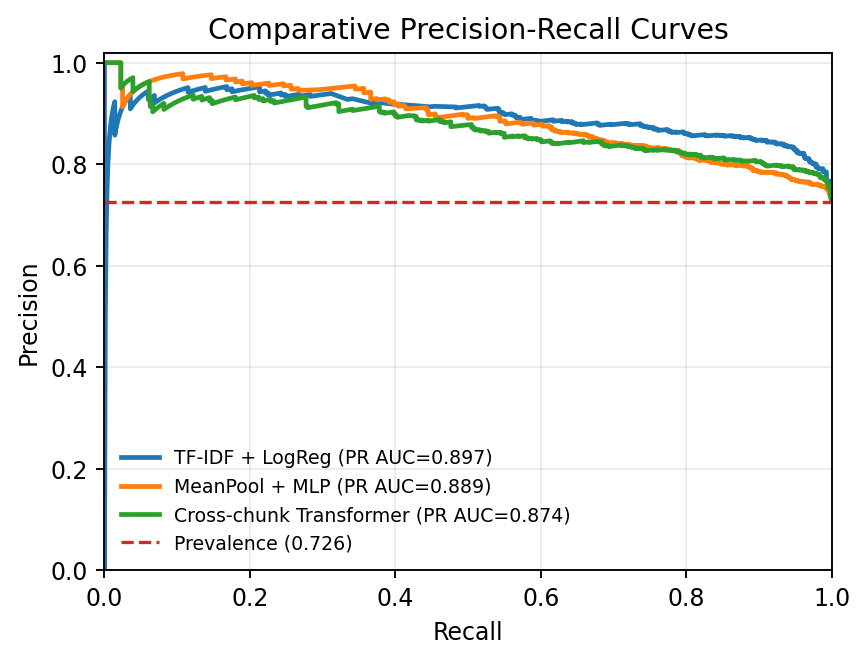
\includegraphics[width=0.94\linewidth]{figures/pr_curve_cv.png}
  \caption{Curvas comparativas de precisión-exhaustividad a partir de predicciones agregadas fuera de pliegue para la línea base léxica más sólida (TF--IDF + regresión logística), la mejor línea base densa con promedio (Promedio + MLP) y el transformer entre fragmentos. La línea horizontal discontinua marca la prevalencia positiva ($\pi \approx 0.726$). TF--IDF muestra en general el mejor compromiso entre precisión y exhaustividad, mientras que ambos modelos basados en LLM permanecen sustancialmente por encima de la referencia sin capacidad predictiva.}
  \label{fig:pr}
\end{figure}

\begin{figure}[t]
  \centering
  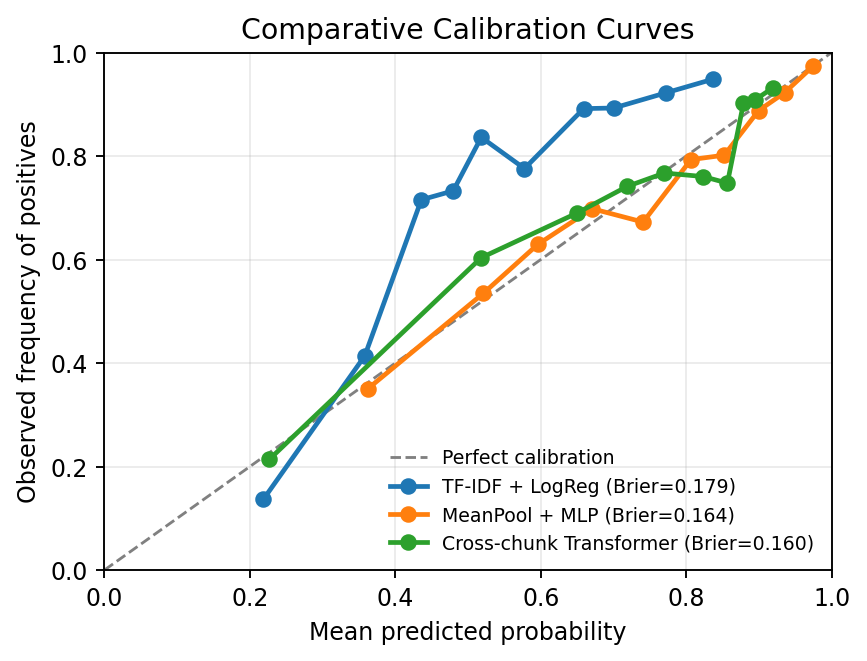
\includegraphics[width=0.94\linewidth]{figures/calibration_curve_cv.png}
  \caption{Curvas comparativas de calibración a partir de predicciones agregadas fuera de pliegue para TF--IDF + regresión logística, Promedio + MLP y el transformer entre fragmentos. La diagonal representa la calibración perfecta. El ordenamiento y la calibración no coinciden: el transformer se mantiene más próximo a una señal probabilística útil y calibrada, mientras que TF--IDF es más sólido como modelo de ordenamiento que como estimador de probabilidades.}
  \label{fig:calibration}
\end{figure}

\begin{figure}[t]
  \centering
  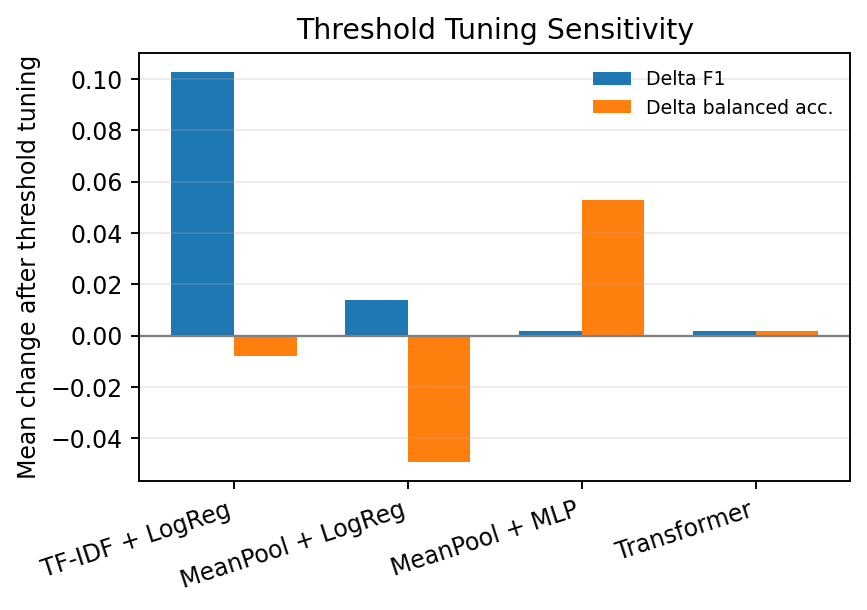
\includegraphics[width=0.94\linewidth]{figures/threshold_sensitivity_comparison.png}
  \caption{Cambio medio en F1 y exactitud balanceada del pliegue de prueba después de sustituir el umbral predeterminado de $0.5$ por el umbral que maximiza F1 en una partición interna de validación. El ajuste mejora considerablemente el F1 de TF--IDF + regresión logística, presenta efectos mixtos en los modelos con promedio y apenas modifica el transformer entre fragmentos, lo que indica una mayor estabilidad del punto operativo.}
  \label{fig:threshold-sensitivity}
\end{figure}


\section{Lectura comparativa por criterio}

\subsection{Ranking}

TF--IDF más regresión logística alcanzó ROC AUC 0,814 y PR AUC 0,899, los mayores valores medios informados. La diferencia con los modelos densos indica que, en el subconjunto procesado, el vocabulario y los bigramas contienen una señal especialmente útil para ordenar procesos exitosos y no exitosos.

Este resultado es compatible con la naturaleza de los PBC. Al pertenecer todos a construcción vial, las variaciones léxicas pueden reflejar plantillas, requisitos o estilos institucionales dentro de un dominio relativamente homogéneo. La explicación es una hipótesis interpretativa, no una atribución causal: el experimento no identifica qué cláusulas producen un desenlace.

El transformer entre fragmentos no superó al promedio con MLP en ranking. Por tanto, los resultados no apoyan la afirmación de que modelar explícitamente relaciones entre fragmentos sea necesario para extraer la mayor parte de la señal densa en esta configuración.

\subsection{Desempeño con umbral 0,5}

El mayor F1 a umbral fijo correspondió al transformer entre fragmentos, con 0,858. Sin embargo, su exactitud balanceada fue 0,636, inferior a la regresión logística con promedio y a TF--IDF. La diferencia revela el efecto de una clase positiva frecuente: un modelo puede obtener F1 alto favoreciendo predicciones positivas y, al mismo tiempo, distinguir peor la clase negativa.

La exactitud balanceada de 0,728 de TF--IDF fue la mayor de la tabla principal. Como promedia la sensibilidad de ambas clases, ofrece una lectura complementaria al F1. Ninguna de las dos métricas debe interpretarse sin especificar la clase positiva y el umbral.

\subsection{Calibración}

El transformer obtuvo el menor Brier, 0,162, seguido por el MLP con promedio, 0,165. TF--IDF, pese a su mejor ranking, obtuvo 0,179. Esta divergencia es esperable: una transformación monótona puede conservar el orden de los ejemplos y cambiar la correspondencia entre puntajes y probabilidades.

La curva de calibración permite observar el comportamiento por intervalos, pero sus puntos no poseen igual cantidad de datos ni intervalos de confianza en la figura actual. La conclusión se restringe a que el transformer produjo la mejor combinación observada bajo Brier y la curva agregada; no se afirma calibración perfecta ni transferencia automática a otra prevalencia.

\section{Análisis de sensibilidad al umbral}

La selección interna del umbral modificó principalmente el F1 de TF--IDF: el incremento medio fue 0,103. Su exactitud balanceada no aumentó en promedio. Esto muestra que maximizar una métrica en validación no garantiza mejorar otra; el objetivo de selección determina el punto operativo.

Para el transformer, las variaciones medias de F1 y exactitud balanceada fueron 0,002. El resultado sugiere estabilidad alrededor de 0,5 en estas particiones. No demuestra que 0,5 vaya a mantenerse como umbral adecuado si cambia la prevalencia de positivos, el costo relativo de falsos positivos y negativos o la institución de origen.

La regresión logística con promedio mejoró ligeramente F1 y redujo exactitud balanceada. El MLP con promedio mantuvo F1 y mejoró exactitud balanceada. Estos patrones justifican presentar deltas por modelo en lugar de una recomendación general de ``ajustar siempre'' el umbral.

\section{Comparación entre hipótesis experimentales}

\subsection{Señal textual frente a controles}

Todos los modelos no triviales superaron a los controles en ROC AUC y PR AUC. Esta evidencia responde afirmativamente, dentro del subconjunto, a la primera pregunta: los PBC contienen señal predictiva sobre la etiqueta operacionalizada.

La evidencia no permite conocer cuánto proviene de contenido técnico, fórmulas administrativas, organismo convocante o año. Un análisis de ablación por secciones y una validación agrupada por institución serían necesarios para separar estas fuentes.

\subsection{Representación léxica frente a densa}

La representación léxica fue superior en ranking, mientras que las densas fueron competitivas y dos de ellas obtuvieron menor Brier. No existe un ganador único para todos los criterios. La selección dependerá del uso: priorización ordenada, clasificación binaria o puntuación probabilística.

Este hallazgo coincide con trabajos de documentos extensos que recomiendan mantener líneas base TF--IDF y evaluar costo además de desempeño \cite{mamakas2022legal,tuteja2023longtext}. El resultado local es particularmente relevante porque el LLM utilizado tiene una escala muy superior a la regresión logística, pero esa escala no produjo el mayor AUC.

\subsection{Interacciones entre fragmentos}

El transformer mejoró calibración respecto de los otros agregadores, pero no ranking. La hipótesis de que las interacciones entre fragmentos aportarían una ventaja general no queda respaldada. Una explicación posible es que el embedding de cada fragmento ya condense suficiente información y el conjunto sea pequeño para aprender interacciones adicionales. Otra posibilidad es que el último token válido no sea el pooling óptimo. Ambas explicaciones requieren experimentos y se formulan como líneas futuras, no como hechos demostrados.

\section{Costo y complejidad experimental}

La comparación de desempeño debe considerar el costo de obtener cada entrada. TF--IDF utiliza el texto extraído y se ajusta con operaciones dispersas. Los modelos densos requieren ejecutar una vez un LLM de 20 mil millones de parámetros sobre fragmentos de hasta 4096 tokens. Esa etapa produjo la principal pérdida técnica del embudo: 680 documentos sin embedding, 671 de ellos por memoria.

Después de generar embeddings, el entrenamiento de agregadores es comparativamente liviano y puede reutilizar los archivos \texttt{.pt}. Sin embargo, una evaluación de extremo a extremo debe contabilizar la codificación inicial y la selección que induce. El mejor Brier del transformer se obtuvo sobre documentos que sí pudieron codificarse; no hay evidencia de su desempeño en los 680 excluidos.

\section{Discusión de resultados}

El hallazgo principal no es que una representación domine universalmente a las demás, sino que diferentes representaciones parecen capturar distintos aspectos de la tarea. TF--IDF más regresión logística ofrece el mejor ordenamiento, lo que sugiere que la señal léxica es muy informativa en este dominio. Esto es plausible porque los documentos de licitación suelen contener fórmulas administrativas repetidas, requisitos estandarizados, terminología específica y expresiones procedimentales que pueden correlacionarse fuertemente con los resultados posteriores. En este contexto, características léxicas dispersas pueden recuperar gran parte de la señal predictiva mediante un modelo lineal relativamente simple.

Esto no debe interpretarse como evidencia contraria a las representaciones basadas en LLM. Todos los modelos no triviales de esta familia permanecen claramente por encima de las líneas base y los embeddings promediados se mantienen próximos al transformer. Ello indica que los embeddings congelados de los fragmentos ya codifican información densa útil. En otras palabras, buena parte del valor del LLM puede residir en la propia representación, más que en la complejidad del mecanismo posterior de agregación.

La comparación entre el promedio y el transformer resulta especialmente informativa. Si las interacciones detalladas entre fragmentos fueran la principal fuente de capacidad predictiva, el transformer debería dominar claramente las líneas base agregadas. Eso no ocurre en los experimentos actuales. El MLP con promedio se aproxima al transformer en ordenamiento y la regresión logística con promedio incluso lo supera en exactitud balanceada. Esto sugiere que el modelado explícito de interacciones aún no proporciona una ventaja clara de ordenamiento bajo el régimen de datos y la señal de supervisión actuales.

No obstante, el transformer conserva una ventaja importante: la calibración y la estabilidad del umbral. Obtiene el mejor puntaje de Brier y muestra muy poca sensibilidad al ajuste del umbral, mientras que TF--IDF más regresión logística se beneficia considerablemente de dicho ajuste en F1. Desde una perspectiva aplicada, esto importa porque el modelo preferido para ordenar no necesariamente es el mismo que se prefiere para priorizar mediante probabilidades o para lograr un comportamiento estable en producción. La naturaleza relativamente estandarizada de los documentos de construcción vial también puede contribuir al buen desempeño de las líneas base léxicas.

Parte de la señal predictiva puede reflejar la complejidad documental, las prácticas institucionales de redacción, la estandarización de procedimientos u otras regularidades textuales latentes. Estas señales son legítimas para la predicción porque están disponibles ex ante, cuando se emite el documento. Sin embargo, no deben interpretarse como causas de los resultados de una contratación.

En conjunto, la comparación resulta informativa incluso sin un único ganador dominante. Para aplicaciones de gobierno y democracia electrónicos, este es precisamente el punto: los sistemas de monitoreo de contrataciones requieren más que un puntaje alto de ordenamiento. También necesitan probabilidades calibradas, líneas base transparentes y umbrales cuyo comportamiento pueda explicarse antes de utilizarlos para priorizar la atención humana. Los resultados muestran que los modelos léxicos son muy competitivos, que los embeddings congelados de LLM ya capturan gran parte de la señal densa útil y que la principal ventaja comparativa del transformer reside en su calibración y estabilidad ante el umbral, no en su desempeño bruto de ordenamiento.


\subsection{Implicaciones para Paraguay}

El resultado más inmediato es metodológico: en PBC paraguayos de construcción vial, una línea base léxica bien configurada debe preceder a modelos más costosos. Esto no implica descartar LLM. Indica que cualquier propuesta basada en ellos debe demostrar una ventaja vinculada al objetivo operativo, como calibración, transferencia o análisis semántico, y no apoyarse únicamente en su complejidad.

Un sistema de apoyo a la DNCP o a un organismo de control podría usar ranking para ordenar expedientes y revisión humana para interpretar causas. Antes de ello sería necesario validar sobre períodos posteriores, incluir organismos no vistos, recuperar PBC faltantes y definir el evento que realmente se desea anticipar. La etiqueta \texttt{complete} frente a estados no exitosos es útil para investigación, pero una política pública puede requerir objetivos más específicos.

La Ley N.º 7021/2022 enfatiza eficiencia, competencia, transparencia e integridad \cite{dncpLey7021}. Una predicción de estado no mide por sí sola esos principios. Cualquier integración institucional debería mantener separadas la señal estadística, la evaluación normativa y la decisión administrativa.

\subsection{Comparación con otros países}

Acikalin et al. encontraron señal predictiva en descripciones de convocatorias \cite{acikalin2024procurementcalls}; este estudio encuentra señal en PBC paraguayos completos. La coincidencia apoya la idea general de que el lenguaje ex ante informa sobre desenlaces, pero no permite equiparar variables objetivo ni magnitudes.

VigIA utiliza metadatos e índices orientados a sobrecostos, demoras e irregularidades en Colombia \cite{salazar2024vigia}. El presente trabajo usa texto y un estado final más amplio. Los enfoques podrían complementarse en el futuro, pero su unión requeriría un conjunto paraguayo donde ambos tipos de variables estén disponibles en el mismo momento.

Los modelos mexicanos centrados en corrupción usan información relacional de compradores y proveedores \cite{aldana2022mexico}. Como el presente experimento no incorpora redes, no puede evaluar esa dimensión. La comparación confirma que ``analítica de contratación'' comprende tareas heterogéneas y que las métricas solo son comparables cuando coinciden etiqueta, momento y población.

\section{Síntesis de hallazgos}

Los hallazgos pueden resumirse de la siguiente forma:

\begin{enumerate}
  \item Los modelos no triviales ordenaron mejor que referencias sin habilidad, lo que evidencia señal textual en el subconjunto.
  \item TF--IDF más regresión logística logró el mejor ranking y la mayor exactitud balanceada de la tabla principal.
  \item El transformer entre fragmentos logró el mejor Brier y el mayor F1 a umbral 0,5.
  \item El promedio de embeddings permaneció cerca del transformer, por lo que no se observó una ventaja general del modelado entre fragmentos.
  \item La optimización de umbral benefició métricas y modelos de manera desigual.
  \item La pérdida de documentos durante recuperación y embedding limita la extrapolación al universo de la DNCP.
\end{enumerate}

Estas conclusiones se restringen a la evidencia observada y servirán de base para el capítulo final.
